% !TeX root = ../../main.tex
\subsection{Dispersion moderation improves BARCS in genome-scale simulation}
\label{sec:crispulator}

We used CRISPulator to evaluate a FACS design under known truth
\citep{nagy2017crispulator}.  At the primary multiplicity of infection
(MOI) of 0.20, three prespecified seeds each generated 10,000 genes, five
guides per gene, four independent replicates, and low, bulk, and high
fractions.  All methods received the same counts and design.

The BARCS comparison isolates guide-dispersion moderation.  BARCS-ST uses the original
guide-specific dispersion estimate, whereas BARCS-MOD moderates those
estimates before applying the same gene summary.  Moderation increased average
precision from 0.902 to 0.919 and F1 at gene FDR 0.10 from 0.811 to 0.847,
while realized FDP remained nearly unchanged (0.065 and 0.066).  This supports
dispersion moderation within the common BARCS pipeline.

\begin{table}[htbp]
\centering
\caption{Genome-scale CRISPulator comparison for the primary three-bin design
at MOI 0.20 (three-seed mean).  Each method
is evaluated at its nominal gene-level threshold; the resulting operating
points are therefore not matched on realized FDP.}
\label{tab:crispulator-comparators}
\small
\begin{tabular}{lrrrr}
\toprule
Method & AUROC & Average precision & Realized FDP & F1\\
\midrule
BARCS-ST & 0.947 & 0.902 & 0.065 & 0.811\\
BARCS-MOD & 0.954 & 0.919 & 0.066 & 0.847\\
MAGeCK-MLE & 0.957 & 0.921 & 0.006 & 0.718\\
CRISPhieRmix & 0.929 & 0.867 & 0.197 & 0.785\\
\bottomrule
\end{tabular}
\end{table}

\begin{figure}[!t]
\centering
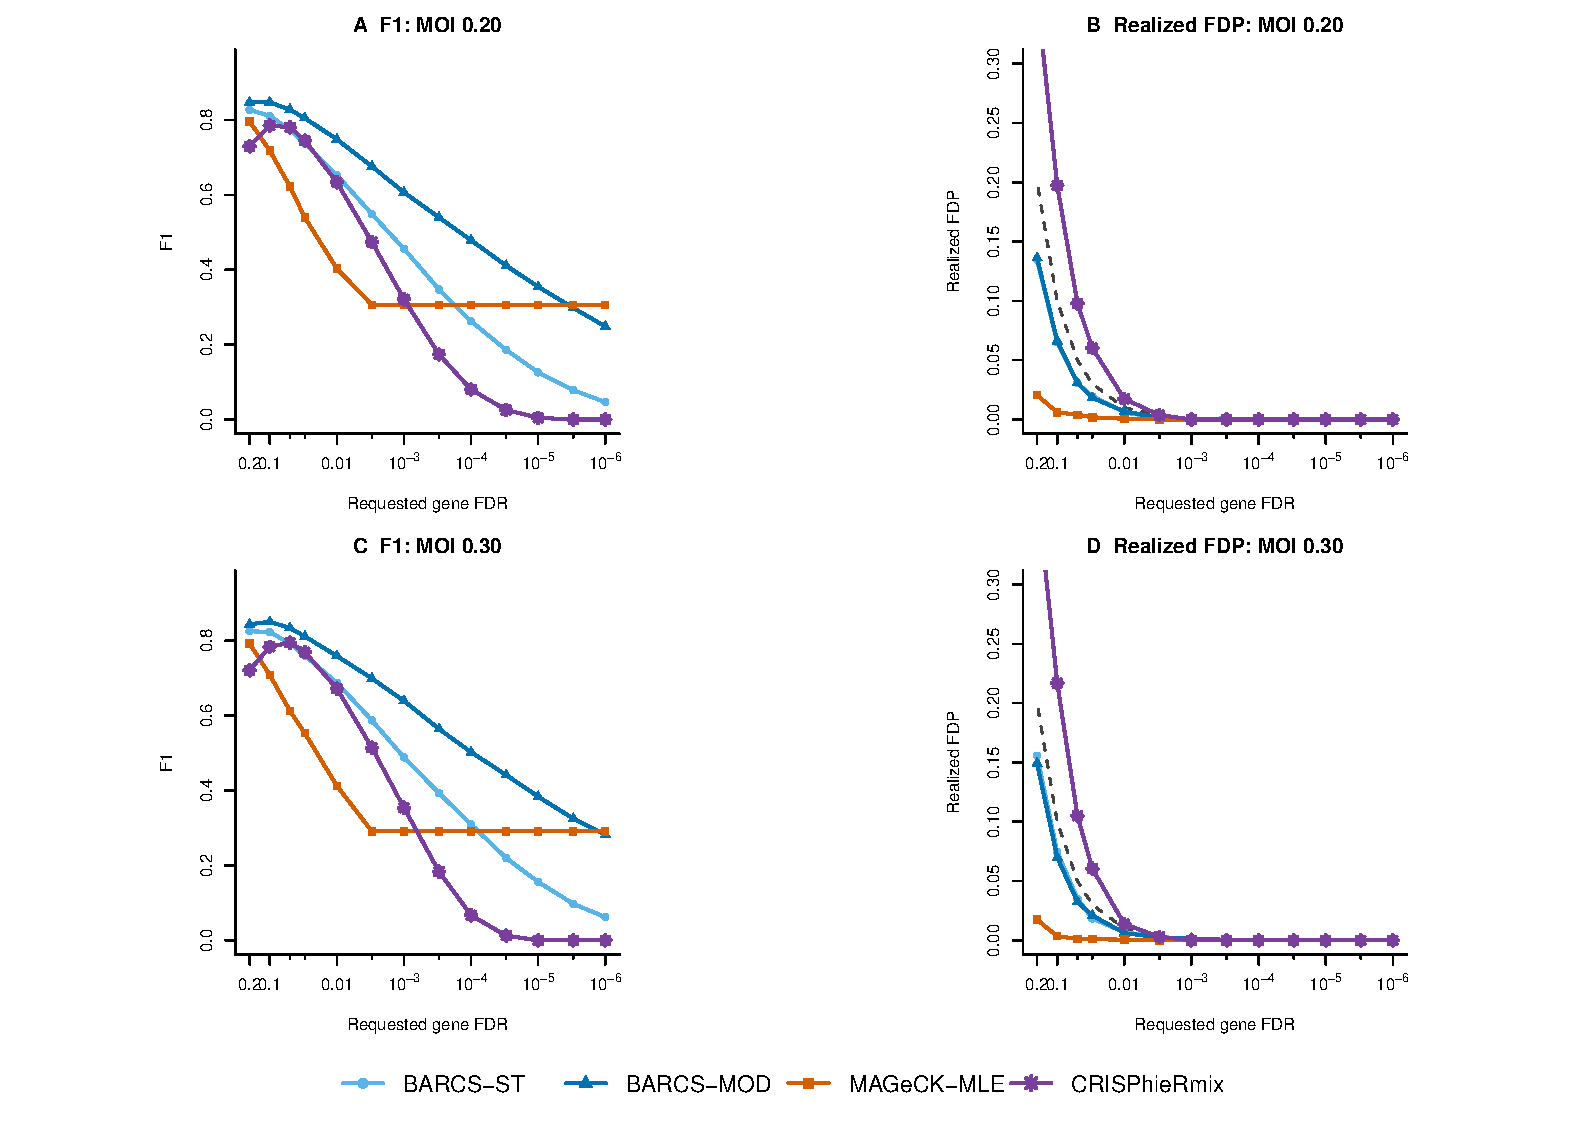
\includegraphics[width=\textwidth]{figures/crispulator_facs_moi_10k_f1_by_fdr.pdf}
\caption{\textbf{CRISPulator threshold sensitivity.}  (A,B) MOI 0.20 and
(C,D) MOI 0.30.  F1 is shown on the left and realized FDP on the right; the
dashed diagonal denotes realized FDP equal to the nominal threshold.  F1 panels use a common y scale, as do realized-FDP panels.
All 13 evaluated thresholds are marked.  BARCS-ST and BARCS-MOD are two settings of one estimator and
therefore share a colour, separated by line type and point shape.  The shared
simulation, gene summary, and thresholds isolate the BARCS-ST versus BARCS-MOD
moderation effect.}
\label{fig:crispulator}
\end{figure}

The moderation gain persisted across requested thresholds at MOI 0.20 and in
the secondary MOI-0.30 analysis (Figure~\ref{fig:crispulator}).  Fitting the
50,000 guide-level regressions required 70.1--102.8 seconds per primary seed
on the analysis system, providing a direct screen-scale runtime check.
MAGeCK-MLE slightly exceeded BARCS-MOD in AUROC and average precision while
operating at a much lower realized FDP; CRISPhieRmix operated at a higher FDP
(Table~\ref{tab:crispulator-comparators}).  These differences limit
comparisons of F1 at a common nominal threshold.  In the broader 400-gene
comparison, edgeR-QL, DESeq2, and limma--voom matched or exceeded BARCS
ranking.  After matching methods on realized FDP, the comparison did not
distinguish the methods above an FDP of 0.005.
